\begin{center}
   {\colorbox{grey2}{
         \begin{minipage}[t]{0.9\textwidth}
\subsubsection*{Scope}
This Pirana Quick Guide explains how blocks of differential equations
defined in \$DES can be converted to differential equations code
that can be used for simulation using R/deSolve, Berkeley Madonna or Matlab.
          \end{minipage}
      }
   }
\end{center}


\subsubsection*{Introduction}
\begin{itemize}
\item If a model contains differential equations as defined in a
  \$DES-block, these may be converted to R/deSolve, Berkeley Madonna
  or Matlab.
\item This can be done by selecting a model, accessing the
  right-mouse-button menu and then selecting \emph{Translate Model}
  (Figure \ref{fig:Fig1}).
\item Next, files will be generated containing code to numerically
  solve these differential equations. The code can be used to perform
  simulations in these software packages.
\item Pirana will automatically extract parameter values and use them
  in the simulation code. If the selected model has already been run
  in NONMEM, it will use the final parameter estimates. If a result
  file is not available, Pirana will use the initial parameter
  estimates. Note that parameter esimates are extracted for fixed
  effects only. 
\item Generated R/deSolve code will be automatically loaded in the
  defined R interface. Berkeley Madonna and Matlab code will be opened
  in the defined code editor. Examples of generated R and Berkeley
  Madonna code are depicted in Figures \ref{fig:Fig2} and \ref{fig:Fig3} respectively.
\item An example of associated simulation output for the R/deSolve
  code is depicted in Figure \ref{fig:Fig4}.  
\end{itemize}

%% Fig 1 - ODE menu
\begin{figure}[h] \centering
    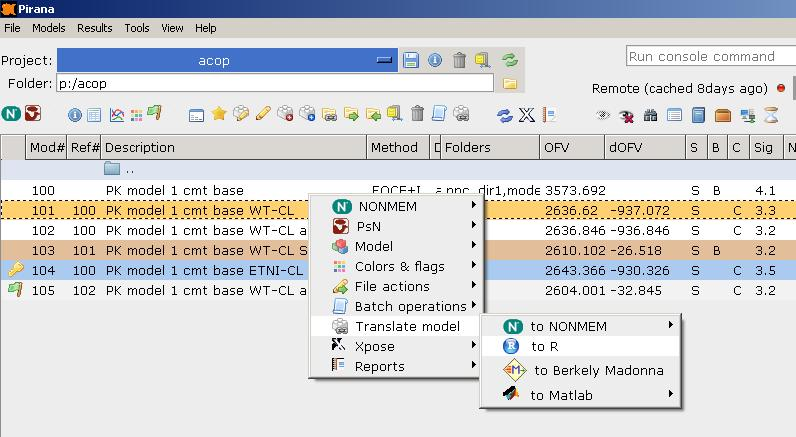
\includegraphics[scale=.4]{images/ODE_1.jpg}
    \caption{Translate options in Pirana \label{fig:Fig1}}
\end{figure}

%% Fig 2 - Generated Madonna code
\begin{figure}[h] \centering
    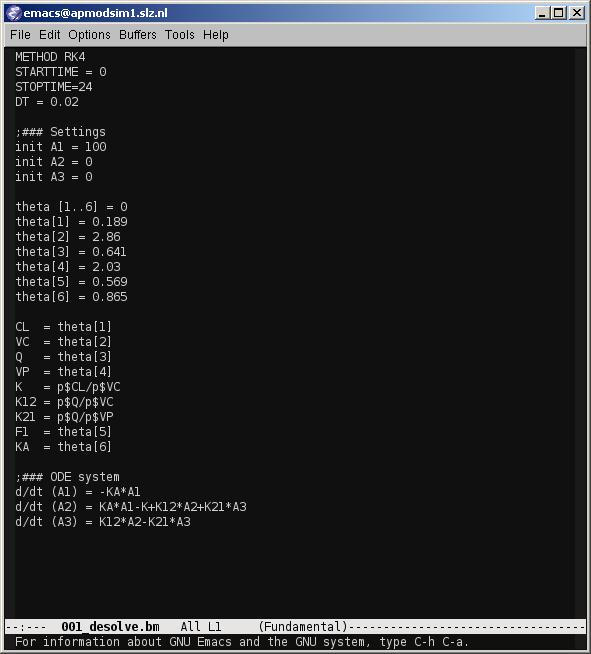
\includegraphics[scale=.5]{images/ODE_2.jpg}
    \caption{Generated BM code \label{fig:Fig2}}
\end{figure}

%% Fig 3 - Generated R code
\begin{figure}[h] \centering
    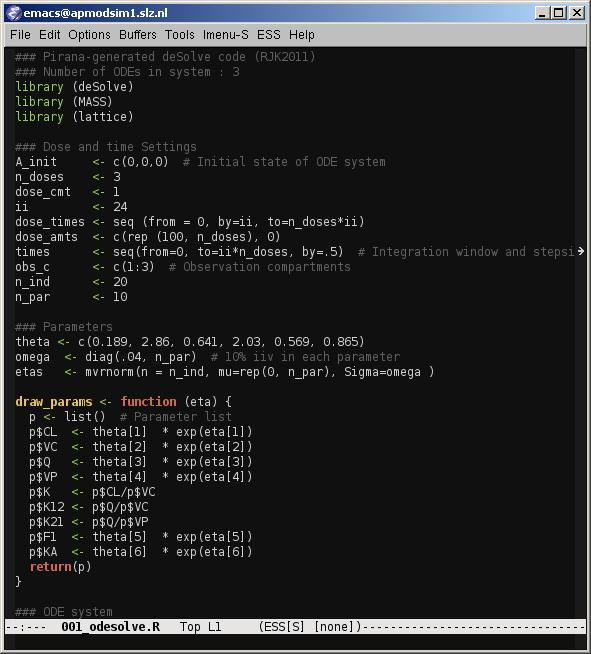
\includegraphics[scale=.5]{images/ODE_3.jpg}
    \caption{Generated R code \label{fig:Fig3}}
\end{figure}

%% Fig 4 - Simulations result R
\begin{figure}[h] \centering
    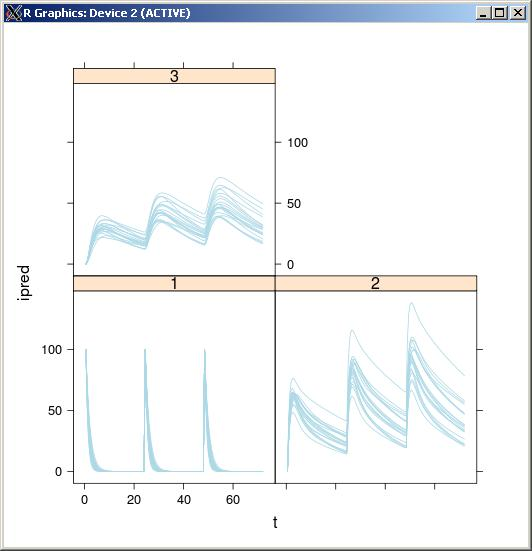
\includegraphics[scale=.4]{images/ODE_4.jpg}
    \caption{Graphical output of simulation R code \label{fig:Fig4}}
\end{figure}
